\documentclass[12pt]{article}
%%%%%%%%%%%%%%%%%%%%%%%%%%%%%
% Preámbulo
% 
\usepackage[T1]{fontenc}
\usepackage[utf8]{inputenc}
\usepackage[spanish]{babel}
\parindent=0cm %Modifica tamaño de sangría.%
\usepackage{amsmath}
\usepackage{amssymb,amsfonts,latexsym,cancel}
%
\usepackage{graphicx}
\usepackage{epstopdf} %convierte el formato eps a pdf%
\usepackage{float} %Permite colocar la imagen el punto que nosotros queremos%
\usepackage{subfigure} %Este paquete permite colocar las figuras en una sola fila%
%%%%%%%%%%%%%%%%%%%%%%%%%%%%%%
\begin{document}
\title{Práctica 4. \\ Gráficas}
\author{Edison Achalma}
\date{14 de marzo de 2021}
\maketitle
\tableofcontents

\section{Incluir gráficas externas}
En \LaTeX podemos incluir figuras externas o generadas directamente en \LaTeX \, utilizando algún paquete, algunos de los formatos que podemos utilizar son \textbf{.png}, \textbf{.eps} y \textbf{.pdf}. \\[0.5cm]
Los formatos vectoriales como los son \textbf{.eps} y \textbf{.pdf} son los más recomendados cuando hacemos gráficas en las cuáles queremos observar detalles y precisión, porque no pierden calidad al aumentar o disminuir su tamaño. Y para imágenes en general podemos utilizar los formatos \textbf{.jpg} o \textbf{.png}

\section{Paquete graphicx}
\includegraphics[scale=1]{imagen1.pdf} \\
%Se pone 1  para que el imagen se suba en formato original%
%Las figuras o imágenes deben estar junto a los codigos o estar en la misma carpeta%
%El imagen se acomoda al lado izquierdo%

Imagen centrada y en escala 0.4
\begin{center}
\includegraphics[scale=0.4]{imagen1.pdf}
\end{center}

\begin{itemize}
\item  scale: Escala de la imagen. \\ Escala de 0.1

\begin{center}
\includegraphics[scale=0.1]{imagen1.pdf}
\end{center}

\item width: Ancho deseado de la imagen en cm. \\ Ancho de 4cm

\begin{center}
\includegraphics[width=4cm]{imagen1.pdf}
\end{center}

\item height: Altura deseada de la imagen en cm. \\ Altura de 5cm
\end{itemize}

\begin{center}
\includegraphics[height=5cm]{imagen1.pdf}
\end{center}

\begin{center}
\includegraphics[scale=0.1]{imagen1.pdf} \quad
\includegraphics[scale=0.2]{imagen1.pdf} \quad
\includegraphics[scale=0.3]{imagen1.pdf} \quad
\includegraphics[scale=0.4]{imagen1.pdf}
\end{center}

\newpage
\section{Objetos flotantes}
En \LaTeX podemos incluir figuras externas o generadas directamente en \LaTeX \, utilizando algún paquete, algunos de los formatos que podemos utilizar son \textbf{.png}, \textbf{.eps} y \textbf{.pdf}. \\[0.5cm]

%Daremos mas propiedades a nuestras figuras%
\begin{figure}[!ht] %[!h] Esta propiedad hace que coloquemos el imagen en donde queremos, [!ht] Esto hace que el latex force en colocar la imagen en la parte superior de la página y [!hb]  forza en colocar la imagen en la parte inferior%
\centering %Este comando centra la figura%
\includegraphics[scale=0.5]{imagenmat.pdf}
\caption{Imagen a escala 0.5} %Descripción del imagen%
\label{figura1}
\end{figure}

Los formatos vectoriales como los son \textbf{.eps} y \textbf{.pdf} son los más recomendados cuando hacemos gráficas en las cuáles queremos observar detalles y precisión, porque no pierden calidad al aumentar o disminuir su tamaño. Y para imágenes en general podemos utilizar los formatos \textbf{.jpg} o \textbf{.png}

%OJO las figuras se pueden poner en una capeta, entonces el comando para incluir figuras cambia en esta forma \includegraphics[scale=0.5]{figuras/imagenmat.pdf} donde figuras representa el nombre de la carpeta%

\begin{itemize}
\item t: La imagen en la parte superior (top).
\item b: La imagen en la parte inferior (bottom).
\item h: La imagen en el sitio que escribimos (here).
\end{itemize}

\begin{figure}[H] %Esta H forza la imagen para poner en el punto que nostros queremos%
\centering
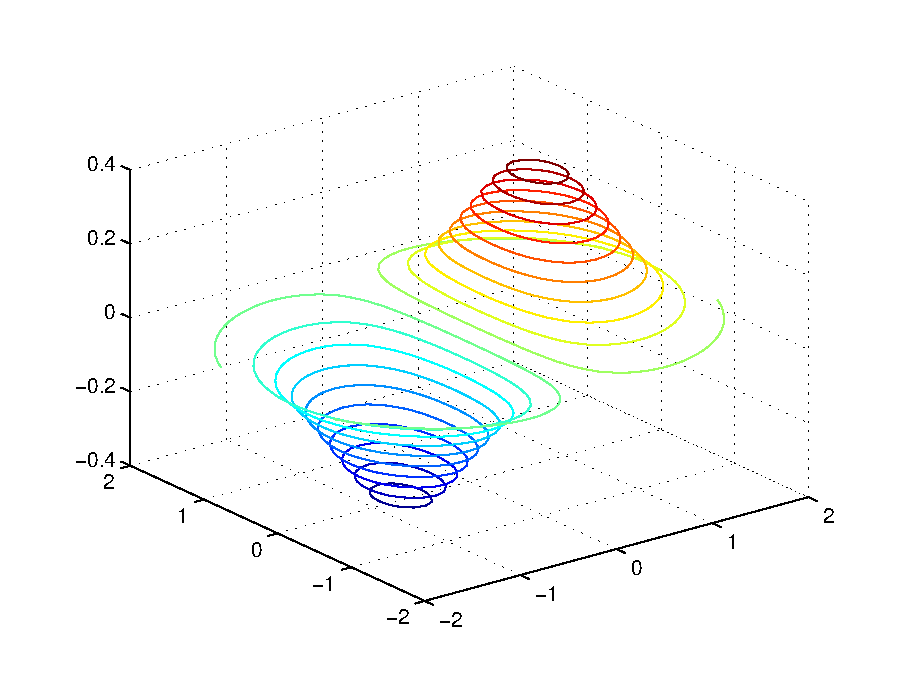
\includegraphics[scale=0.5]{figuras/imagenmat2.eps}
\caption{Imagen en formato eps} %Descripción del imagen%
\label{figura1}
\end{figure}

\subsection{Paquetes float}

\begin{figure}[H]
\centering
\includegraphics[scale=0.3]{figuras/elefante.jpg}
\caption{Imagen en formato jpg} %Descripción del imagen%
\label{figura2} %RECORDAR que LABEL es para nombrar el objeto y luego sive para hacer la refrencia%
\end{figure}

Como los muestra la imagen \eqref{figura2} \\
En \LaTeX podemos incluir figuras externas o generadas directamente en \LaTeX \, utilizando algún paquete, algunos de los formatos que podemos utilizar son \textbf{.png}, \textbf{.eps} y \textbf{.pdf}. \\[0.5cm]
Los formatos vectoriales como los son \textbf{.eps} y \textbf{.pdf} son los más recomendados cuando hacemos gráficas en las cuáles queremos observar detalles y precisión, porque no pierden calidad al aumentar o disminuir su tamaño. Y para imágenes en general podemos utilizar los formatos \textbf{.jpg} o \textbf{.png}

\begin{figure}[H]
\centering
\includegraphics[scale=0.15]{figuras/Petirrojo2.jpg}
\caption{Imagen en formato jpg}
\label{figura3} 
\end{figure}

\subsection{Paquete subfigure}

Este paquete permite colocar las figuras en una sola fila.

\begin{figure}[!ht]
\centering
\subfigure[Primera figura]
{\includegraphics[scale=0.1]{figuras/Petirrojo2.jpg}}
\quad
\subfigure[Segunda figura]
{\includegraphics[scale=0.1]{figuras/Petirrojo2.jpg}}
\quad
\subfigure[Tercera figura]
{\includegraphics[scale=0.1]{figuras/Petirrojo2.jpg}}
\caption{Varias figuras con subfigure}
\label{figurasvarias} 
\end{figure}
Tal como aparece en la figura anterior \eqref{figurasvarias}.

\section{Comando put}
Ahora usaremos el comando put \\ Este comando permite añadir símbolos, ecuaciones o textos en la figura.

\begin{figure}
\includegraphics[scale=0.5]{imagenmat.pdf} 
\put(-270,110){usando el comando put}
\put(-180,30){$x+1$}
\caption{Imagen a escala 0.5}
\label{figura1.1}
\end{figure}

Ahora los textos un poco mas pequeños con el comando footnotesize{}

\begin{figure}
\includegraphics[scale=0.5]{imagenmat.pdf} 
\put(-270,110){\footnotesize{usando el comando put}}
\put(-180,30){$x+1$}
\caption{Imagen a escala 0.5}
\label{figura1.1}
\end{figure}






\end{document}